\documentclass[11pt]{article}
\usepackage{times}
\usepackage{fullpage}
\usepackage{url}
\usepackage{hyperref}
\usepackage{fancyhdr}
\usepackage{graphicx}
\usepackage{enumitem}
\usepackage{subcaption}
\usepackage{amsmath, amsfonts, amsthm, fouriernc}
\usepackage{IEEEtrantools}
\usepackage{parskip}
\usepackage{xcolor}
\usepackage{units}
\newcommand{\Fin}[1]{\textcolor{green!50!black}{#1}}  % input amplitude
\newcommand{\Kdc}[1]{\textcolor{red!50!black}{#1}}    % DC gain
\newcommand{\Tc}[1]{\textcolor{blue!50!black}{#1}}    % time constant

\pagestyle{fancy}
\addtolength{\headheight}{2em}
\addtolength{\headsep}{1.5em}
\lhead{\large{ME 2801}}
\rhead{\large{Solutions}}

\usepackage{sectsty}
\sectionfont{\fontsize{12}{8}\selectfont}

\begin{document}

\begin{center}
  \Large{\bf{Solutions: Transfer Functions and Modeling}}
\end{center}

\begin{figure}[h!]
  \centering
  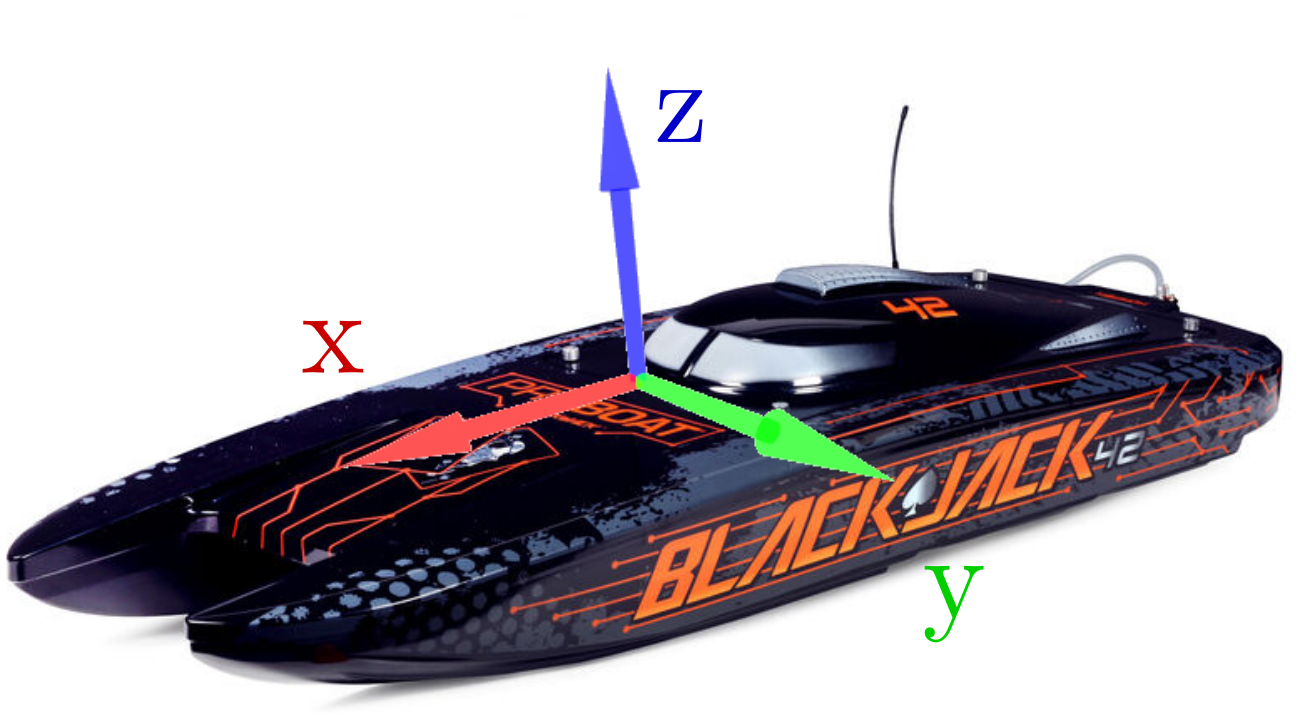
\includegraphics[width=0.25\linewidth]{images/blackjack_cs.png}
  \label{fig:blackjack_cs}
\end{figure}

% ---------------------------------------------------------------
\section*{USV Model}

Parameters: $m = \unit[5.0]{kg}$, $b_x = \unit[8.0]{N\cdot s/m}$, $I = \unit[0.8]{kg\cdot m^2}$, $b_r = \unit[1.2]{N\cdot m\cdot s/rad}$, $N_\delta = \unit[2.0]{N\cdot m/rad}$.

\begin{enumerate}[start=6]

\item Surge equation of motion (Newton's second law along $x$, thrust minus linear drag):
\[
  \boxed{m\,\dot{v}_x(t) + b_x\,v_x(t) = F(t)}
  \qquad\Rightarrow\qquad
  5.0\,\dot{v}_x + 8.0\,v_x = F
\]
Dividing by $b_x$ puts it in standard first-order form, which identifies the time constant and DC gain:
\[
  \underbrace{\Tc{\frac{m}{b_x}}}_{\Tc{\tau}}\,\dot{v}_x + v_x = \underbrace{\Kdc{\frac{1}{b_x}}}_{\Kdc{K_{dc}}}\,F
  \qquad\Rightarrow\qquad
  \Tc{0.625}\,\dot{v}_x + v_x = \Kdc{0.125}\,F
\]
Color key: \Fin{input amplitude}, \Kdc{DC gain}, \Tc{time constant}.

\item With $v_x(0) = 0$ and a step of amplitude $\Fin{F_0} = \unit[\Fin{12}]{N}$, $F(s) = \Fin{F_0}/s$:
\[
  V_x(s) = \frac{\Kdc{K_{dc}}\,\Fin{F_0}}{s\,(\Tc{\tau}\,s + 1)} = \frac{\Kdc{0.125}\cdot\Fin{12}}{s\,(\Tc{0.625}\,s + 1)} = \frac{1.5}{s} - \frac{1.5}{s + 1/\Tc{0.625}}
\]
\[
  \boxed{\begin{aligned}
    v_x(t) &= \Kdc{K_{dc}}\,\Fin{F_0}\left(1 - e^{-t/\Tc{\tau}}\right) = (\Kdc{0.125}\cdot\Fin{12})\left(1 - e^{-t/\Tc{0.625}}\right)\ \unit{m/s} \\
           &= 1.5\left(1 - e^{-t/\Tc{0.625}}\right)\ \unit{m/s}
  \end{aligned}}
\]
\begin{itemize}[nosep]
  \item Plot: first-order rise from 0 toward $\unit[1.5]{m/s}$ with time constant $\Tc{\tau} = \Tc{m/b_x} = \unit[\Tc{0.625}]{s}$.  (Both mass and drag set the time constant, i.e., how quickly the vessel accelerates.)
  \item Steady-state speed: $v_{ss} = \Kdc{K_{dc}}\,\Fin{F_0} = \Kdc{0.125}\cdot\Fin{12} = \unit[1.5]{m/s}$.  (Top speed depends only on drag, $\Kdc{K_{dc}} = \Kdc{1/b_x}$, not on mass.)
  \item 95\% of steady state at $t \approx 3\Tc{\tau} \approx \unit[1.9]{s}$.
\end{itemize}

\item Surge transfer function, thrust to surge velocity:
\[
  \boxed{\begin{aligned}
    G_x(s) = \frac{V_x(s)}{F(s)} &= \frac{1}{m s + b_x} = \frac{\Kdc{1/b_x}}{\Tc{\frac{m}{b_x}}\,s + 1} = \frac{\Kdc{K_{dc}}}{\Tc{\tau}\,s + 1} \\
                                 &= \frac{\Kdc{0.125}}{\Tc{0.625}\,s + 1} = \frac{1}{5.0\,s + 8.0} = \frac{0.2}{s + 1.6}
  \end{aligned}}
\]
\begin{itemize}[nosep]
  \item Units: $V_x/F$ in $\unit{(m/s)/N}$.
  \item Pole at $s = -1/\Tc{\tau} = \unit[-1.6]{s^{-1}}$.
  \item DC gain $\Kdc{K_{dc}} = \Kdc{1/b_x} = \unit[\Kdc{0.125}]{(m/s)/N}$.
\end{itemize}

\item Yaw equation of motion (moment balance about $z$, rudder moment minus linear drag):
\[
  \boxed{I\,\dot{r}(t) + b_r\,r(t) = N_\delta\,\delta(t)}
  \qquad\Rightarrow\qquad
  0.8\,\dot{r} + 1.2\,r = 2.0\,\delta
\]

\item Yaw-rate transfer function, rudder to yaw rate:
\[
  \boxed{\begin{aligned}
    G_r(s) = \frac{R(s)}{\Delta(s)} &= \frac{N_\delta}{I s + b_r} = \frac{\overbrace{N_\delta/b_r}^{K_{dc}}}{\underbrace{(I/b_r)}_{\tau}\,s + 1} = \frac{K_{dc}}{\tau\,s + 1} \\
                                    &= \frac{1.67}{0.667\,s + 1} = \frac{2.0}{0.8\,s + 1.2} = \frac{2.5}{s + 1.5}
  \end{aligned}}
\]
\begin{itemize}[nosep]
  \item Units: $R/\Delta$ in $\unit{(rad/s)/rad}$.
  \item Time constant $\tau = I/b_r = 0.8/1.2 = \unit[0.667]{s}$; pole at $s = -1/\tau = \unit[-1.5]{s^{-1}}$.
  \item DC gain $K_{dc} = N_\delta/b_r = 2.0/1.2 = \unit[1.67]{(rad/s)/rad}$.
\end{itemize}

\item Heading transfer function.  Since $r = \dot{\psi}$, $R(s) = s\,\Psi(s)$ (zero initial heading), so heading adds an integrator:
\[
  \boxed{G_\psi(s) = \frac{\Psi(s)}{\Delta(s)} = \frac{N_\delta}{s\,(I s + b_r)} = \frac{2.0}{s\,(0.8\,s + 1.2)} = \frac{2.5}{s\,(s + 1.5)}}
\]
Units: $\Psi/\Delta$ in $\unit{rad/rad}$; poles at $s = 0$ and $s = \unit[-1.5]{s^{-1}}$.

\item With $\Delta(s) = 0.3/s$, the final value theorem gives
\[
  r_{ss} = \lim_{s \to 0} s\,G_r(s)\,\frac{0.3}{s} = \frac{2.5}{1.5}(0.3)
  \quad\Rightarrow\quad
  \boxed{r_{ss} = \unit[0.5]{rad/s}}
\]
(about $\unit[28.6]{deg/s}$).  The heading $\psi(t)$ grows without bound, so the vessel turns in a circle.

\end{enumerate}

\end{document}
